\documentclass[withoutpreface,bwprint]{cumcmthesis} % 去除承诺书和编号页
\title{校门开放方式对于通行效率的影响探究}

\begin{document}
\maketitle
\begin{abstract}
本文旨在探究校门开放方式对学生通行效率的影响。
通过排队论的方法,建立了三种不同复杂度的模型来分析和比较两种开门模
式:默认开门和默认关门。首先,我们简化了模型,假设非高峰期单校门情
形下的随机服务时间为固定数值,构建了模型1。接着,模型2引入了负指数
分布来更细致地描述服务时间。最后,模型3综合考虑了高峰期和非高峰期,
多校门情形以及顾客流在不同队列中的转移概率,是最符合实际的模型。

为了构建排队论基本模型,对服务规则与顾客源建立随机性模型。
在服务规则分析中,我们考虑了刷卡时间和经过时间的波动性,并采用负
指数分布来描述校门的服务过程。顾客源分析则区分了学生和其他人员,分
别建立了适用于高峰期和非高峰期的泊松流模型。此外,还考虑了步行与单
车两种不同的出行方式,并对刷卡成功率进行了建模。

理论分析部分,我们使用了排队论的基本公式和概率论,得到了描述系统运
行特征的差分方程,然后求得了稳态解,并通过状态转移图的方式进行可视化。
对于不同的模型,分别通过Pollaczek-Khintchine公式
和Little法则,计算了平均队长和平均等待时间,并将数值模拟时
用到的参数代入公式。定性的来说,各模型中均可以表示默认关门的通行效率
要低于默认开门的模式。定量的来说,对于单通道模型下的默认开门的平均队长
与默认关门的平均队长的比值,确定服务型为0.52,随机服务型为0.42.

数值模拟部分,我们采用了元胞自动机模型和蒙特卡洛法,对排队-通行过程进行了精细模拟
,并进行了统计分析以验证理论解的正确性。元胞自动机分别模拟单通道与多通道
的情况,在多通道时,设置转移概率,有效模拟真实过程,并进行可视化展示。
统计结果时,使用10000个时间步长下的平均队列作为评价指标,
模拟100次,对结果进行统计分析,最后在$95\%$的置信度下,
给出两者平均队长之比的置信区间为[0.4516,0.4526],与理论结果的定性结果一致,
在具体的定量分析上有有一定差距。
\par 考虑实际情况,在单通道随机模型的基础上建立多通道随机模型,重要的特征是
行人可以以一定的概率换道,从而更快的通过校门。在高人流量和低人流量的情况下分别对
单通道和多通道模型进行数值模拟,得到平均队长。模拟结果显示,多通道可以显著减少
平均队长,同时在多通道、成功率较高的情况下,两种开门方式下的通行效率相差不大。
考虑到校园管理对于安全性的需求,结合模拟结果,给出不同场景下的开门方式建议。
\par 最后,在模型建立完成的基础上对模型进行评价与展望。
本文讨论了模型的优缺点,并提出了改进方向,包括实地调研获取参数、选择更
符合实际的模型以及将模型推广到更多场景。

\keywords{排队论\quad 通行方式 \quad 元胞自动机 \quad 泊松过程}
\end{abstract}
\section{模型建立与求解}

\subsection{基本理论}
\subsubsection{服务系统的规则设定}
    首先从理论上,基于排队论的基本公式与概率论相关知识,在理论上对两种开门模型
    进行理论计算,得到平均队长与平均等待时间作为评价通行效率的指标。

    从顾客源的角度来说,顾客源的输入为泊松过程,泊松过程的概率表达式如下

    \begin{equation}
        P_n(t)=\frac{e^{-\lambda t}(\lambda t)^n}{n!},t>0,n \in \mathbb{N}
    \end{equation}
    $\lambda$表示单位时间内平均到达的顾客数,
    对于非高峰期与高峰期的顾客源,分别使用不同的$\lambda_l,\lambda_h$来描述。

    按照泊松过程的概率公式,随机生成顾客队列,
    并让队列以$v_f=1 m/s$的速度前进。

    对于到达校门的人,开始进行服务。服务时间由固定服务时间与随机服务时间相加得到,
    即$t_{all}=2t_{c}+t_{r}$。$t_r$服从负指数分布,概率密度与分布函数如下:
    \begin{equation}
        \begin{aligned}
            f(t) &=\mu e^{-\mu t},  \\
            F(t) &=1-e^{-\mu t},t>0
        \end{aligned}
    \end{equation}

    求的随机服务时间$t_r$的数学期望$E(t_r)=\frac{1}{\mu}$即为平均随机服务时间,
    因此$\mu$的意义就是单位时间内的平均服务人数,也就是校门的平均通过速率。
    在加上固定服务时间$2t_c$,得到总服务时间的数学期望$E(t_{all})=2t_c+\frac{1}{\mu}$,
    方差$ Var(t_{all})=Var(t_r)=\frac{1}{\mu^2}$。
    对于精度要求不高的模型,也可以使用一个常数(平均服务时间)来代替,
    即数学期望$E(t_{all})=2t_c+\frac{1}{\mu}$,
    方差$ Var(t_{all})=0$。

    有了顾客源与服务时间的随机分布模型,可以服务定义强度
    $\rho=\lambda E(t_{all})=2t_c \lambda+\frac{\lambda}{\mu}$

    在这里假设服务强度$\rho<1$,而这个假设也是合理的,因为否则会导致队伍长度发散。
    使用排队论中的经典公式Pollaczek-Khintchine公式,对于一个任意分布的服务时间T,
    且规定对应分布的服务强度$\rho=\lambda E(t_{all})$,有
    \begin{equation}
        L_s=\rho +\frac{\rho^2 +\lambda^2 Var(T)}{2(1-\rho)}
    \end{equation}
    根据Little法则,可以对平均服务长度与平均等待时长进行换算
    \begin{equation}
        L_s=\lambda W_s
    \end{equation}

    基于以上理论分析,给出我们模型的理论平均队长与理论平均等待时间,
    在考虑随机服务时间为定值的条件下
    \begin{equation}
        \begin{aligned}
            L_s & =\rho +\frac{\rho^2 }{2(1-\rho)} \\
            W_s &=\frac{\rho}{\lambda} +\frac{\rho^2}{2\lambda (1-\rho)}
        \end{aligned}
    \end{equation}
    在考虑随机服务时间为负指数分布的条件下
    \begin{equation}
        \begin{aligned}
            L_s & =\rho +\frac{\rho^2 +\lambda^2 /\mu^2}{2(1-\rho)} \\
            W_s &=\frac{\rho}{\lambda} +\frac{\rho^2 +\lambda^2 /\mu^2}{2\lambda (1-\rho)}
        \end{aligned}
    \end{equation}
\subsubsection{求解方法}
为了细致的分析这一过程,我们需要求解得到系统的运行特征$P_n(t)$,
它表示系统在任意时刻t系统中有n个人的概率。

为方便后续的描述,将平均服务时间简写为$\frac{1}{\mu}$,实际为$2t_c+\frac{1}{\mu}$。

先在t时刻与$t+\Delta t$时刻之间的时间段内进行研究。由于在任意时间段内
一个顾客到达的概率与t无关,所以有一个顾客到来的概率为$\lambda \Delta t$,
与之对应,没有顾客到来的概率为$1- \lambda \Delta t$。

由于此时将服务时间简化为定值,所以这段时间内一个顾客离去的概率为$\mu \Delta t$,
没有顾客离去的概率为$1-\mu \Delta t$。

发生两个以上顾客到来或者离去的概率为以上两个概率的平方,所以是$o(\Delta)t$,可以忽略不计。

接下来,在t时刻与$t+\Delta t$时刻之间的时间段内,可能发生四种情况,
\begin{itemize}
\item 一个人到来,一个人离去,概率为$\lambda \Delta t \cdot \mu \Delta t$,结果为人数加1。
\item 一个人到来,没有人离去,概率为$\lambda \Delta t \cdot (1-\mu \Delta) t$,结果为人数不变。
\item 没有人到来,一个人离去,概率为$(1-\lambda \Delta) t \cdot \mu \Delta t$,结果为人数减1。
\item 没有人到来,没有人离去,概率为$(1-\lambda \Delta t) \cdot (1-\mu \Delta) t$,结果为人数不变。
\end{itemize}


再考虑在时刻t时,有n-1,n,n+1个顾客时的情形,要想在时刻$t+\Delta t$时有n个人,
只有三种情况(不考虑两个人以上的变动),
\begin{itemize}
\item 在时刻t有n个人,在接下来$\Delta t$时间段内人数不变。
\item 在时刻t有n-1个人,在接下来$\Delta t$时间段内人数加1。
\item 在时刻t有n+1个人,在接下来$\Delta t$时间段内人数减1。 
\end{itemize}


综合得到以下状态转移概率公式:
\begin{equation}
    P_n(t+\Delta t)=P_n(t)(1-\lambda \Delta t-\mu \Delta t)+P_{n+1}(t)(\mu \Delta t) +P_{n-1}(t)(\lambda \Delta t)+o(\Delta t)
\end{equation}

在这个状态转移概率公式中对t取极限,得到关于$P_n(t)$差分微分方程:
\begin{equation}
    \frac{d P_n(t)}{dt}=\lambda P_{n-1}(t)+\mu P_{n+1}(t)-(\lambda+\mu )P_n(t)
\end{equation}

我们只关心系统状态的稳态解,而不关心系统状态的瞬态解,所以只考虑$P_n$,而不是$P_n(t)$。

从而得到一个关于稳态状态之间的差分方程:
\begin{equation}
    \begin{aligned}
        & \lambda P_{n-1}(t)+\mu P_{n+1}(t)-(\lambda+\mu )P_n(t)=0,n\geq 1 \\
        & -\lambda P_{0}+\mu P_{1}=0
    \end{aligned}
\end{equation}

以上的差分方程是很好求解的,由于顾客源于排队的空间都设置为无穷大,所以可以解得:
\begin{equation}
    \begin{aligned}
        P_0 &=1-\rho \\
        P_n &=(1-\rho)\rho^n,n\geq1
    \end{aligned}
\end{equation}
其中的$\rho=\frac{\lambda}{\mu}$,它的物理意义为服务强度。

从而可以得到$L_s$的数学期望$L_s=\frac{\rho}{1-\rho}$,这与
基本理论中的Pollaczek-Khintchine公式结果是一致的。

\subsection{单通道确定性模型}
\subsubsection{理论分析}
首先考虑非高峰期的情况下,使用一个参数为$\lambda_{l}$的泊松过程来表示顾客源,
使用一个常数(平均服务时间)来代替负指数分布的随机服务时长,即$M/D/1/\infty/\infty/FCFS$模型。

使用上述方法得到一个关于稳态状态之间的差分方程:
\begin{equation}
    \begin{aligned}
        & \lambda P_{n-1}(t)+\mu P_{n+1}(t)-(\lambda+\mu )P_n(t)=0,n\geq 1 \\
        & -\lambda P_{0}+\mu P_{1}=0
    \end{aligned}
\end{equation}

这个差分方程表示的各个不同状态之间的转移关系,可以用状态转移图来表示:
\begin{figure}[ht]    
    \centering
    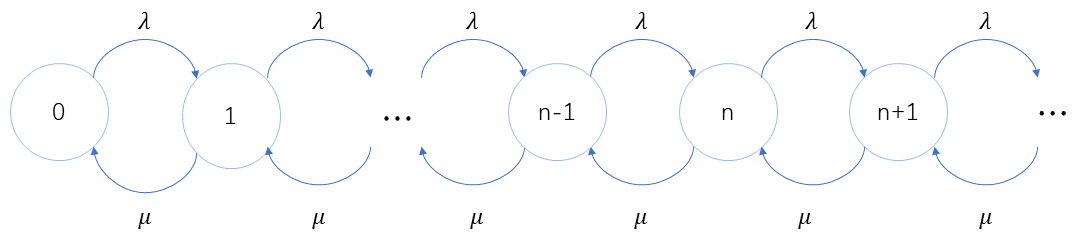
\includegraphics[width=.7\textwidth]{images/transform1.PNG}
    \caption{单通道状态转移图}
    \label{fig:transform1}
\end{figure}
\par 对于默认关门的情况,服务时间的均值$E(t_1)=2t_c+\frac{1}{\mu}$,
方差$Var(t_1)=0$
所以服务强度$\rho_1=2t_c\lambda_l+\frac{\lambda_l}{\mu}$,
由于将服务时间设置为确定值,所以直接使用Pollaczek-Khintchine公式进行求解。
得到理论上的平均队长$L_s=\rho_1+\frac{\rho_1^2}{2(1-\rho_1)}$。
\par 同理,对于默认开门的情况,服务时间是$t_2=t_r+t_{penal}$,
$t_{penal}$表示刷卡失败的惩罚时间,
随机变量$t_{penal}$可以用以下概率公式描述
\begin{equation}
    p(t_{penal})=
    \begin{cases}
        1-p_o,t_{penal}=T_{penal} \\
        p_o,t_{penal}=0
    \end{cases}
\end{equation}
其中$p_o$为开门成功率。$T_{penal}$为惩罚的具体时间大小。
这里的$t_r$与$t_{penal}$是相互独立的,因为后者是否存在仅仅取决于是否刷卡失败,
而这对随机服务时间,即刷卡时间与经过时间,没有任何影响。从而得到总服务时间的期望与方差如下:
\begin{equation}
    \begin{aligned}
        E(t_2) &=\frac{1}{\mu}+(1-p_o)T_{penal} \\
        Var(t_2)&=\frac{1}{\mu^2}+p_o(1-p_o)T_{penal}^2
    \end{aligned}
\end{equation}

所以服务强度$\rho_2=\lambda_l (1-p_o)T_{penal}+\frac{\lambda_l}{\mu}$,
直接运用Pollaczek-Khintchine公式得到理论上的平均队长
$L_s=\rho_2+\frac{\rho_2^2+\lambda^2/\mu^2+\lambda^2 p_o(1-p_o)T_{penal}^2}{2(1-\rho_2)}$
\par 最后将两者比较,得到两种服务方式的平均队长的比值
\begin{equation}
    \begin{aligned}
        \frac{L_{s1}}{L_{s2}}&=\frac{\rho_1+\frac{\rho_1^2}{2(1-\rho_1)}}{\rho_2+\frac{\rho_2^2+\lambda_l^2/\mu^2+\lambda_l^2 p_o(1-p_o)T_{penal}^2}{2(1-\rho_2)}} \\
        &=\frac{(2\rho_1-\rho_1^2)(1-\rho_2)}{(1-\rho_1)[2\rho_2-\rho_2^2+\lambda_l^2/\mu^2+\lambda_l^2 p_o(1-p_o)T_{penal}^2]}
    \end{aligned}
\end{equation}
其中$\rho_1=2t_c\lambda_l+\frac{\lambda_l}{\mu}$,
$\rho_2=\lambda_l (1-p_o)T_{penal}+\frac{\lambda_l}{\mu}$

接下来对结果进行简单的讨论:
\begin{itemize}
    \item 对于服务强度,$\rho_1-\rho_2=\lambda_l(2t_c-(1-p_o)T_{penal})$,
    由于$p_o$是一个很大的值,一般在0.9以上,所以默认关门的服务强度
    比默认关门要大得多,即在人流相同的条件下,默认开门的通行压力要更小。
    \item 对于这个公式,给出我们接下来数值时使用的参数,代入公式进行计算,
    具体取值如下:$t_c=0.5$,$\mu=1$,$p_o=0.9$,$T_{penal}=1$,$\lambda_l=0.2$,
    则$\rho_1=0.4,\rho_2=0.22$,从而$L_{s1}=\frac{3.2}{6},L_{s2}=0.278,\frac{L_{s1}}{L_{s2}}=1.9>1$。
    所以一般默认开门的平均队长是默认关门平均队长的0.52倍。
    也可以根据Little法则算出对应的等待时间比值,与平均队长的比值是一致的。
\end{itemize}

\subsubsection{模型建立}
\par 将校门前的道路网格化,假设行人占据一个网格、自行车占据两个网格。
根据假设,自行车在通过校门的时候会下车推行,
从而行人和自行车在门前的前进速度可以认为相同,设为$1m/s$。
对排队人群进行离散模拟,在每个模拟时间段内,如果行人或自行车前方空格
没有被占用,则前进一格。根据这样的模拟规则,将一个网格的长度设为$1m$。
\par 考虑单通行道的情况,模型可视化展示在图\ref{fig:one-lane-model}中。
\begin{figure}[ht]
    \centering
    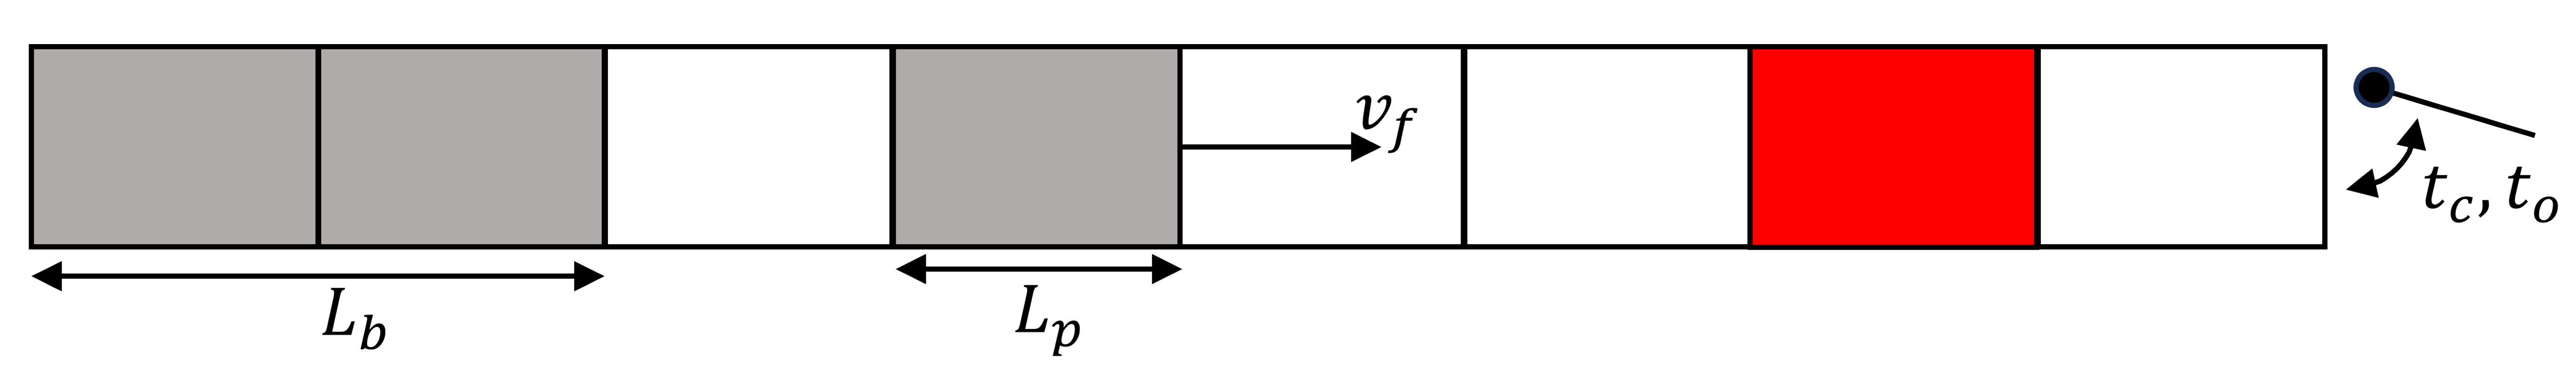
\includegraphics[width=0.6\textwidth]{images/cellular_automata_1_lane.png}
    \caption{单通行道模型可视化,其中灰色块表示网格被占用,红色块表示
    该通行者会刷卡失败(或没有校园卡),图中最右部分为校门}
    \label{fig:one-lane-model}
\end{figure}
\newline 其中:
\begin{itemize}
    \item $L_p, L_b$分别表示行人和自行车占用的网格长度
    \item $v_f$表示行人和自行车的前进速度
    \item $t_o, t_c$分别表示校门的开关时间,考虑实际情况,认为$t_c=t_o$
    \item $t_g,t_p$(图中未标注)分别为刷卡时间和通过时间,在确定性模型中
    两者视为定值
\end{itemize}
人和自行车均在道路最左边生成,道路有最大长度,当道路最左侧已经被占用时,
不再生成人。认为人的生成过程是一个泊松过程,对于高人流量和低人流量的时间段
泊松过程的参数取值不同。
\par 刷卡进校过程的拆分及两种开门方式的不同展示在图\ref{fig:process-entering-gate}中。
\begin{figure}[ht]    
    \centering
    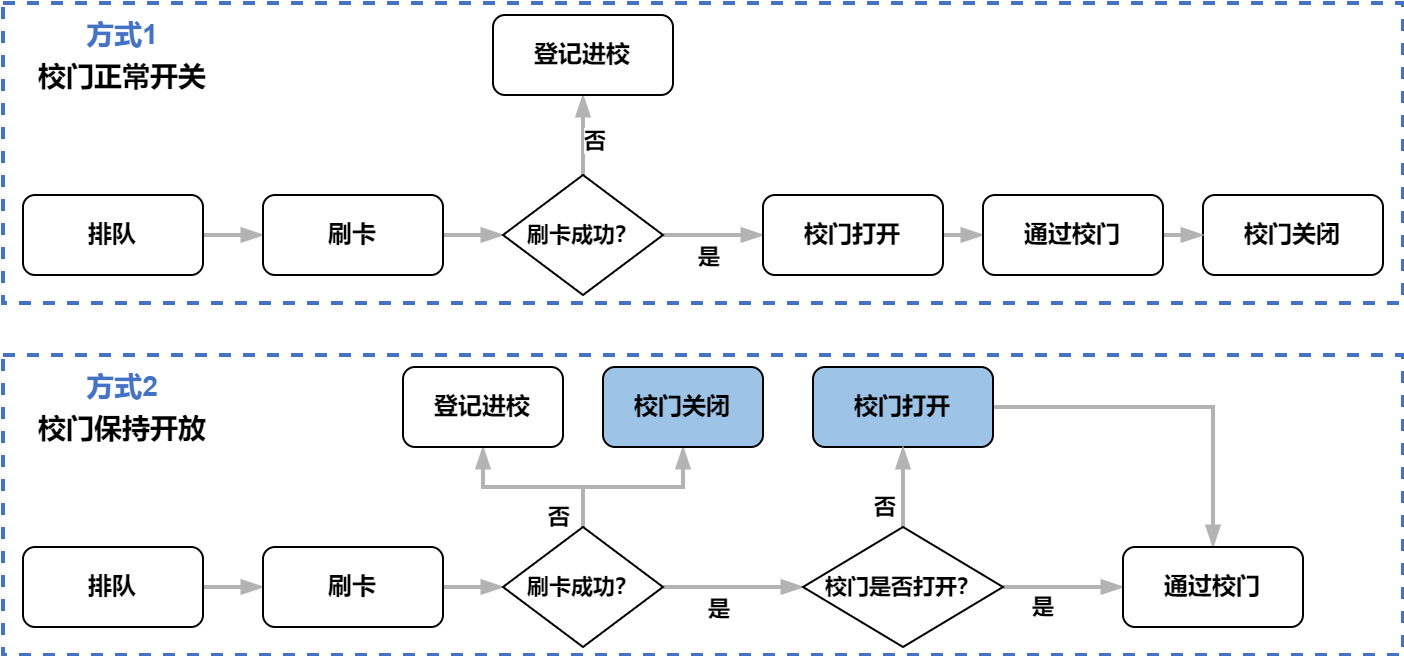
\includegraphics[width=.7\textwidth]{images/enter_gate_process.png}
    \caption{刷卡进校过程及两种校门开关方式的异同}
    \label{fig:process-entering-gate}
\end{figure}
在刷卡进校时,对于两种方法做相应的时间消耗分析:
\begin{itemize}
    \item 门保持开放:
    \begin{itemize}
        \item 如果刷卡成功,直接通过校门,需要的时间即为通过校门的时间加上
        刷卡识别的时间$t_p+t_g$。如果上一个人刷卡失败,该时间变为$t_g+t_o+t_p$。
        \item 如果刷卡失败,需要等待门关闭。根据实际生活经验,刷卡失败
        的个体在刷卡过程中一般花费时间也较长(例如询问在哪里刷身份证),同时
        刷卡失败之后,一般要离开队伍,然后登记入校。
        将这两个过程中时间的消耗合计为
        $t_{penal}$,从而刷卡失败消耗的时间为刷卡时间、等待门关闭的时间和
        离开队伍的时间加和$t_g+t_c+t_{penal}$。
    \end{itemize}
    \item 门正常开关:
    \begin{itemize}
        \item 如果刷卡成功,等待门开放后通过校门,下一个在队伍中的人等待门
        关闭后继续刷卡通过。从而一个人需要的时间为$t_g+t_o+t_p+t_c$。
        \item 如果刷卡失败,需要离开队伍。门正常开关时,不用等待门关闭,
        从而所需时间为$t_g+t_{penal}$。
    \end{itemize}
\end{itemize}

\subsubsection{数值模拟}
模拟的时间步长$t^*$取为$0.5s$,根据实际生活经验,约定开门的时间$t_o=t^*$、
行人的刷卡时间$t_g=t^*$、通过时间$t_p=t^*$、门关上的时间$t_c=t_o=t^*$。
如果刷卡失败,耽误的时间$t_{penal}=2t^*$。根据模型分析:
\begin{itemize}
    \item 门保持开放:
    \begin{itemize}
        \item 刷卡成功:耗时$t_p+t_g=2t^*$。
        \item 刷卡失败:耗时$t_g+t_c+t_{penal}=4t^*$。
    \end{itemize}
    \item 门正常开关:
    \begin{itemize}
        \item 刷卡成功:耗时$t_g+t_o+t_p+t_c=4t^*$。
        \item 刷卡失败:耗时$t_g+t_{penal}=3t^*$
    \end{itemize}
\end{itemize}

设置好以上参数以后,进行10000次模拟,每个两个时间步长$t^*$取样一次,
设置队列容量为40,如果在模拟过程中,队列长度很少达到40,则表示符合队列容量无穷大的假设。

将取样结果展示,得到时间步长曲线,用于观察不同模式下,
系统队列长度随时间变化的趋势,定性评价两个模式的通行效率。
\begin{figure}[ht]    
    \centering
    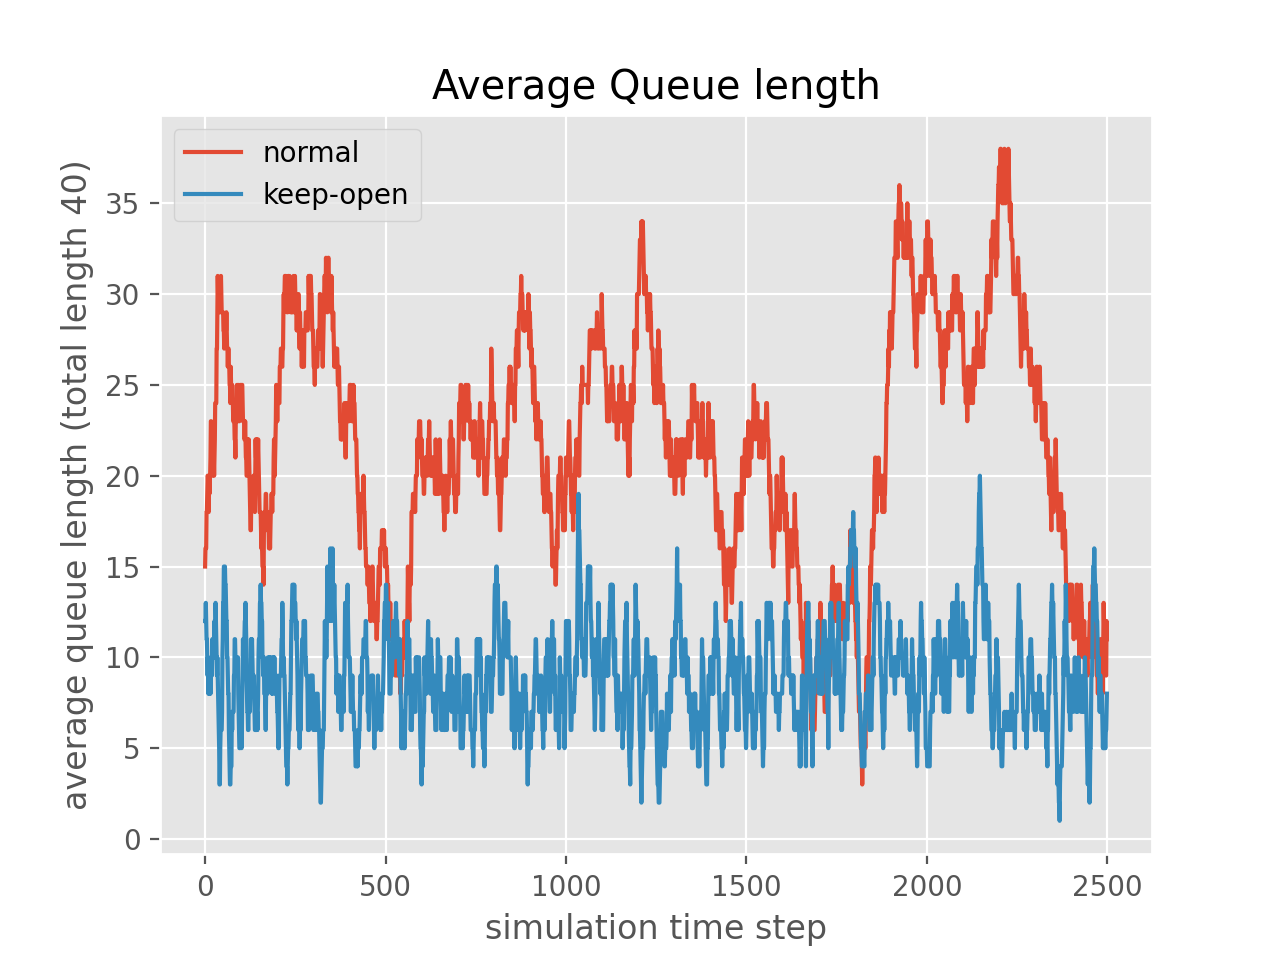
\includegraphics[width=.7\textwidth]{images/队长-时间曲线.png}
    \caption{单通道确定性模型队长-时间曲线}
    \label{fig:queue-length-time}
\end{figure}
从图中可以看出,红色曲线代表现有正常开门方式,即默认关门;蓝色曲线代表默认关门。
从整体上看,红色曲线几乎动在蓝色曲线上方,可以看出默认开门的模式通行效率较高。

为了定量描述两个模式效率的差距,绘制两模式队长比值-时间曲线,
即$\frac{L_{s1}}{L_{s2}}-t$的关系。这个比值是通过对100000次取样的
队长取平均得到的平均队长,从而能够使得队长的比值趋于稳定。通过观察图像
与定量的数值分析,根据统计学知识,按照置信度为$\alpha=0.90$,计算得到
对应置信区间[0.4516,0.4526]。而上文中理论计算得到的比值为0.52,
可以得出两种模式下,理论分析的定性结论与实验一致,但定量结果略有偏差。
\begin{figure}[ht]    
    \centering
    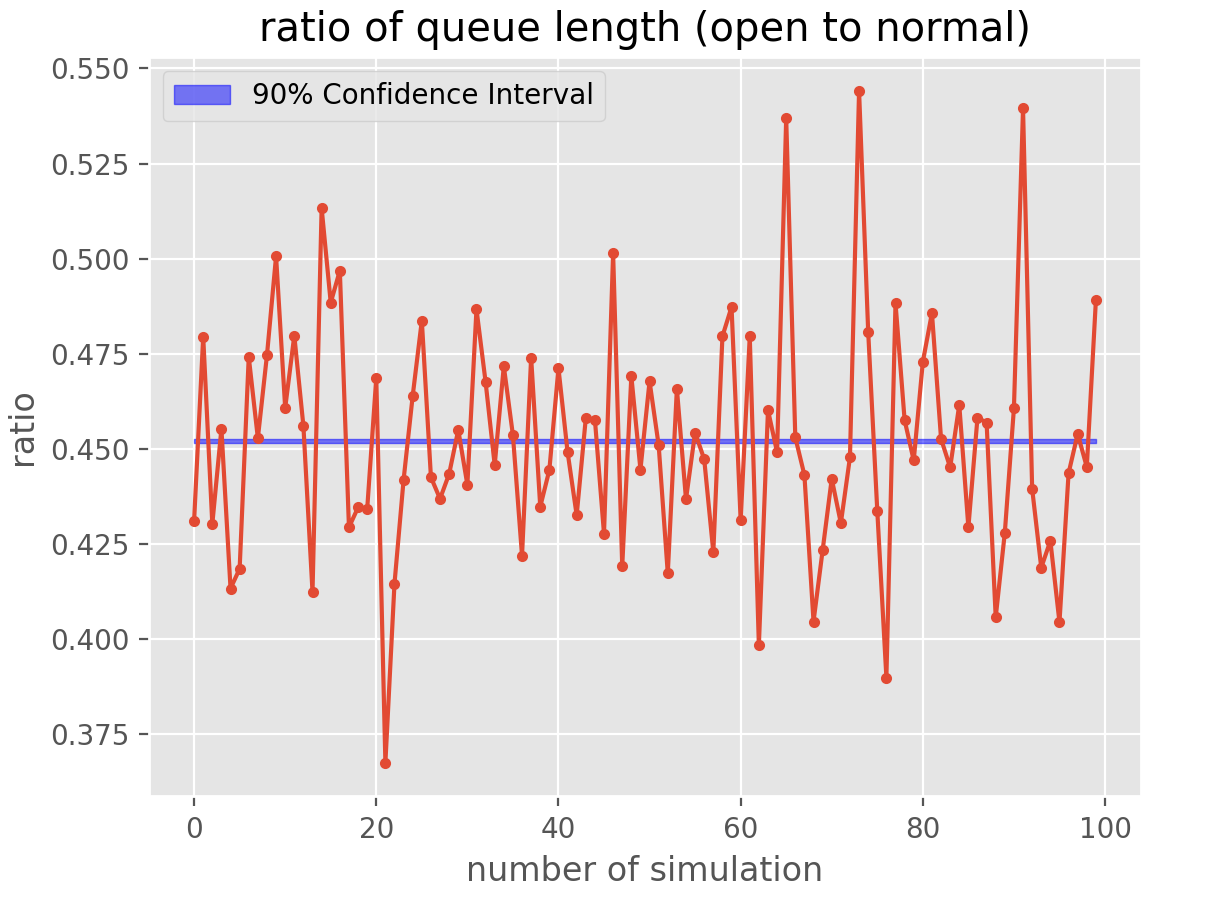
\includegraphics[width=.7\textwidth]{images/队长比例-时间曲线.png}
    \caption{单通道确定性模型两模式队长比值-时间曲线}
    \label{fig:length ratio-time curve}
\end{figure}


\subsection{单通道随机性模型}
\subsubsection{理论分析}
考虑非高峰期的情况下,使用一个参数为$\lambda_{l}$的泊松过程来表示顾客源,
使用负指数分布的随机服务时长,即$M/G/1/\infty/\infty/FCFS$模型。
其中使用的是G而不是M是因为总的服务时长$t_{all}=2t_{c}+t_{r}$,是一个
符合负指数分布的变量加上一个常量,并不是严格的负指数分布,所以用一般分布G表示。

\par 对本模型的求解,主要按照按模型1的求解方法,先建立对应稳态之间的差分方程:
\begin{equation}
    \begin{aligned}
        & \lambda P_{n-1}(t)+\frac{\mu}{2t_c\mu+1} P_{n+1}(t)-(\lambda+\frac{\mu}{2t_c\mu+1} )P_n(t)=0,n\geq 1 \\
        & -\lambda P_{0}+\frac{\mu}{2t_c\mu+1} P_{1}=0
    \end{aligned}
\end{equation}
求解这个差分方程可以得到对应状态的概率
\begin{equation}
    \begin{aligned}
        P_0 &=1-\rho \\
        P_n &=(1-\rho)\rho^n,n\geq1
    \end{aligned}
\end{equation}
其中的$\rho=2\lambda t_c+\frac{\lambda}{\mu}$,它的物理意义为服务强度。

随后,通过与模型1类似的方法可以得到对应状态转移关系。

以下是不同状态转移关系:
\begin{figure}[ht]
    \centering
    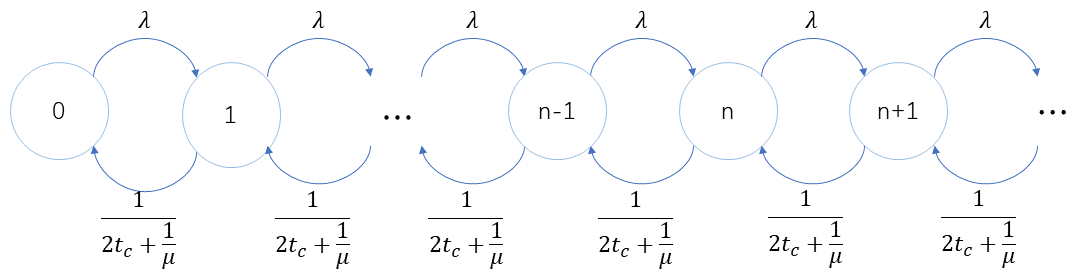
\includegraphics[width=.6\textwidth]{images/transform2.PNG}
    \caption{随机模型单通道状态转移图}
    \label{fig:transform2}
\end{figure}

\par 对于默认关门的情况,服务时间是$t_1=2t_c+\frac{1}{\mu}$,
所以服务强度$\rho_1=2t_c\lambda_l+\frac{\lambda_l}{\mu}$,
得到理论上的平均队长$L_s=\frac{\rho_1}{1-\rho_1}$。
\par 同理,对于默认开门的情况,服务时间是$t_2=t_r+t_{penal}$,
$t_{penal}$表示刷卡失败的惩罚时间,惩罚时间的建模与上一个模型一致。

其中$p_o$为开门成功率。$T_{penal}$为惩罚的具体时间大小。
这里的$t_r$与$t_{penal}$是相互独立的,因为后者是否存在仅仅取决于是否刷卡失败,
而这对随机服务时间,即刷卡时间与经过时间,没有任何影响。从而得到总服务时间的期望与方差如下:
\begin{equation}
    \begin{aligned}
        E(t_2) &=\frac{1}{\mu}+(1-p_o)T_{penal} \\
        Var(t_2)&=\frac{1}{\mu^2}+p_o(1-p_o)T_{penal}^2
    \end{aligned}
\end{equation}

所以服务强度$\rho_2=\lambda_l (1-p_o)T_{penal}+\frac{\lambda_l}{\mu}$,
直接运用Pollaczek-Khintchine公式得到理论上的平均队长
$L_s=\rho_2+\frac{\rho_2^2+\lambda^2/\mu^2+\lambda^2 p_o(1-p_o)T_{penal}^2}{2(1-\rho_2)}$
\par 最后将两者比较,得到两种服务方式的平均队长的比值
\begin{equation}
    \begin{aligned}
        \frac{L_{s1}}{L_{s2}}&=\frac{\frac{\rho_1}{1-\rho_1}}{\rho_2+\frac{\rho_2^2+\lambda_l^2/\mu^2+\lambda_l^2 p_o(1-p_o)T_{penal}^2}{2(1-\rho_2)}} \\
        &=\frac{2\rho_1(1-\rho_2)}{(1-\rho_1)[2\rho_2-\rho_2^2+\lambda_l^2/\mu^2+\lambda_l^2 p_o(1-p_o)T_{penal}^2]}
    \end{aligned}
\end{equation}
其中$\rho_1=2t_c\lambda_l+\frac{\lambda_l}{\mu}$,
$\rho_2=\lambda_l (1-p_o)T_{penal}+\frac{\lambda_l}{\mu}$

接下来对结果进行简单的讨论:
\begin{itemize}
    \item 对于服务强度,$\rho_1-\rho_2=\lambda_l(2t_c-(1-p_o)T_{penal})$,
    由于$p_o$是一个很大的值,一般在0.9以上,所以默认关门的服务强度
    比默认关门要大得多,即在人流相同的条件下,默认开门的通行压力要更小。
    \item 对于这个公式,给出我们接下来数值时使用的参数,代入公式进行计算,
    具体取值如下:$t_c=0.5$,$\mu=1$,$p_o=0.9$,$T_{penal}=1$,$\lambda_l=0.2$,
    则$\rho_1=0.4,\rho_2=0.22$,从而$L_{s1}=\frac{2}{3},L_{s2}=0.278,\frac{L_{s1}}{L_{s2}}=2.4>1$。
    所以一般默认开门的平均队长是默认关门平均队长的0.42倍。
    也可以根据Little法则算出对应的等待时间比值,与平均队长的比值是一致的。
\end{itemize}

\subsubsection{模型建立}
在确定性模型中,刷卡时间和通行时间(之后统称为服务时间)认为是常数,
在实际情况中,服务时间往往会因为客户对象的不同而发生变化\footnote{
    例如,由于老年人的刷卡时间和通过时间相较年轻人明显较长,
    所以老年人的服务时间将会明显长于年轻人。
}。选择利用负指数分布刻画这种服务时间的不确定性,从而更好地刻画队伍的运动情况。


\subsection{多通道模型}
\subsubsection{理论分析}
考虑非高峰期与高峰期的情况下,使用参数为$\lambda_{l},\lambda_{h}$的泊松过程来表示顾客源,
使用负指数分布的随机服务时长,考虑多通道且允许相互转移的过程,这个相互转移的发生条件是:
假设人流自发流向长度最短的队伍,
即$M/G/3/C_{queue}/C_{source}/FCFS$模型。

设置服务站数c=3,这会影响到差分方程的建立与求解过程。

以下是不同状态转移关系:
\begin{figure}[ht]    
    \centering
    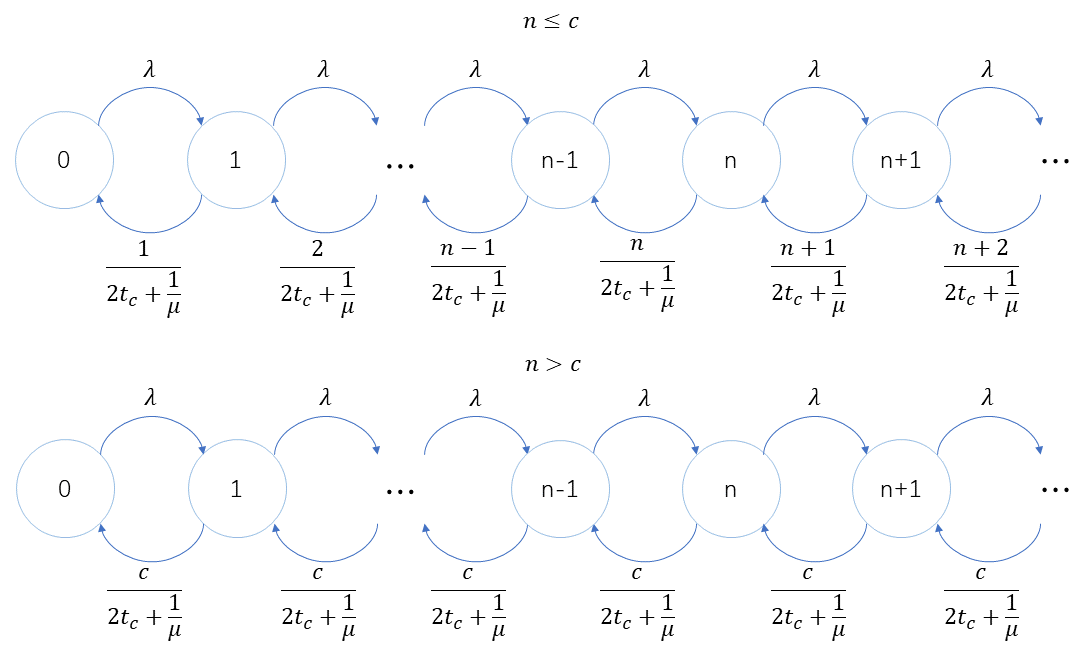
\includegraphics[width=.6\textwidth]{images/transform3.PNG}
    \caption{多通道状态转移图}
    \label{fig:transform3}
\end{figure}

对于非高峰期的多通道模型,
对应的差分方程模型如下:
\begin{equation}
    \begin{aligned}
        &\mu P_1=\lambda P_0 \\
        &(n+1)\mu P_{n+1}+\lambda P_{n-1}=(\lambda+n\mu)P_n, 1\leq n\leq c \\
        &c\mu P_{n+1}+\lambda P_{n-1}=(\lambda +c\mu )P_n, n>c
    \end{aligned}
\end{equation}

其中的$\rho=\frac{\lambda}{\mu}\geq 1$,否则队长会发散。
求解结果如下:
\begin{equation}
    \begin{aligned}
        &P_0=\Big[\sum_{k=0}^{c-1}\frac{1}{k!} \rho^k +\frac{1}{c!(1-\rho)}\cdot \rho^c \Big]^{-1} \\
        &P_n=
        \begin{cases}
            \frac{1}{n!}\rho^n P_0 \\
            \frac{1}{c!c^{n-c}}\rho^n P_0
        \end{cases}
    \end{aligned}
\end{equation}

从而求得平均对长$L_s=\frac{(c\rho)^c\rho}{c!(1-\rho)^2}P_0+\rho$

对于高峰期的多通道模型,
对应的差分方程模型如下:
\begin{equation}
    \begin{aligned}
        &\mu P_1=\lambda P_0 \\
        &(n+1)\mu P_{n+1}+\lambda P_{n-1}=(\lambda+n\mu)P_n, 1\leq n\leq c \\
        &c\mu P_{n+1}+\lambda P_{n-1}=(\lambda +c\mu )P_n, n>c
    \end{aligned}
\end{equation}

其中的$\rho=\frac{\lambda}{\mu}\geq 1$,否则队长会发散。
由于队列的容量有限,用$N=C_{queue}$,所以有限制$\sum_{k=0}^{N}P_k=1$
求解结果如下:
\begin{equation}
    \begin{aligned}
        &P_0=\Big[\sum_{k=0}^{c}\frac{1}{k!} (c\rho)^k +\frac{c^c\rho (\rho^c-\rho^N)}{c!(1-\rho)} \Big]^{-1} \\
        &P_n=
        \begin{cases}
            \frac{1}{n!}(c\rho)^n P_0 \\
            \frac{c^c}{c!}\rho^n P_0
        \end{cases}
    \end{aligned}
\end{equation}

从而求得平均对长$L_s=\frac{(c\rho)^c\rho}{c!(1-\rho)^2}P_0[1-\rho^{N-c}-(N-c)\rho^{N-c}(1-\rho)]+c\rho (1-\rho)$
多通道模型的非高峰期与高峰期理论求解完毕。

\subsubsection{模型建立}
\par 实际情况中,往往有多条入校通道。相较于单通道,多通道的引入,使得
行人和自行车在条件允许时,可以选择更换通道,从而更快地通过校门。
在实际情况中,如果当前通道有人刷卡失败



\begin{thebibliography}{9}%宽度9
\bibitem[1]{20120118}
刘延柱.
\newblock 关于摩擦碰撞的Kane难题\allowbreak[J/OL].
\newblock 力学与实践, 2012, 34\penalty0 (1):\penalty0 91-94.
\newblock \url{https://lxsj.cstam.org.cn/cn/article/doi/10.6052/1000-0879-20120118}.

\bibitem[2]{doi:10.1098/rspa.2013.0497}
COHEN~C, DARBOIS-TEXIER~B, DUPEUX~G, et~al.
\newblock The aerodynamic wall\allowbreak[J/OL].
\newblock Proceedings of the Royal Society A: Mathematical, Physical and Engineering Sciences, 2014, 470\penalty0 (2161):\penalty0 20130497.
\newblock \url{https://royalsocietypublishing.org/doi/abs/10.1098/rspa.2013.0497}.

\bibitem[3]{20130314-2}
刘延柱.
\newblock 再论Kane难题\allowbreak[J/OL].
\newblock 力学与实践, 2013, 35\penalty0 (3):\penalty0 77-79.
\newblock \url{https://lxsj.cstam.org.cn/cn/article/doi/10.6052/1000-0879-12-170}.

\end{thebibliography}

\end{document}